% !TeX spellcheck = en_US
\section{Adaptation Strategies}
\label{sec:726_adaptationstrategy}
The previous sections describe the architecture of \ac{VAS} and the concepts necessary for quality- and content-aware adaptation for video streaming.
This section describes the proposed \ac{VAS} adaptation schemes, beginning with an optimal adaptation model that relies on global knowledge.
The proposed \ac{MILP} model guarantees stable quality with minimal data traffic.

Also, two adaptation heuristics are realized, which help \ac{MPEG} \ac{DASH} clients to adapt: 1) \ac{TQA} and 2) the \ac{SQA}.
The \ac{TQA} implies that a \ac{MPEG} \ac{DASH} client specifies a minimum level of quality regarding the \ac{MOS} for the streaming session.
\ac{VAS} calculates an adaptation plan over different video shots, maintaining exactly the specified level of quality with only minimal fluctuations.
This adaptation plan can be device-specific, i.e., including a certain maximum resolution, frame rate, or a specific set of encodings.
To adapt across multiple \ac{MPEG} \ac{DASH} representations, the \acf{SQA} adapts as covertly as possible.
\ac{SQA} is introduced in Section~\ref{sec:726_smooth_adaptation}.
\subsection{Optimal Adaptation}
\label{sec:726_optimalAdaptation}
To determine what is potentially possible, the proposed adaptation heuristics are compared with an optimal adaptation scheme having global knowledge.
An optimal adaptation scheme is formulated for a single playback device, in the form of an \ac{MILP} that extends the work of Hossfeld et al.~\cite{Hossfeld2015a}.
In comparison to their work, we focus on a model for \ac{MPEG} \ac{DASH} and we do not leverage the advantages of \ac{MVLC}.
Furthermore, our aim of the proposed model is very different, as it stabilizes the perceived quality level and minimizes the data traffic generated.
It aims at streaming the lowest bit rate representation, which provides the maximum quality.

As a result, a two-step optimization approach finds a solution that achieves a video adaptation aimed at a target quality level (\ac{MOS}) with minimal switching. 
The aim of the first optimization is to maximize the streamed video quality $W$ for a streaming session represented by the \ac{MPEG} \ac{DASH} segments that are received at the client ($i=1 .. n$) and for the representations of the \ac{MPEG} \ac{DASH} video ($j=1..r_{max}$).
The objective to maximize the quality of a streaming session $W$ is formulated as: 
\begin{equation}
\label{optQual:formula1}
max(W = \sum\limits_{i=1}^{n}\sum\limits_{j=1}^{r_{max}} w_{ij} * x_{ij}) \quad\quad where\quad x_{ij} \in \{0,1\}
\end{equation}
The weight $w_{ij}$ represents the \ac{MOS} value of the representation $j$ and segment $i$.
In this optimization model, it is assumed that the representations for a segment index $i$ are in an ascending order with respect to their perceived quality (\ac{MOS}). 

In additions, conditions are applied to the optimization model:
\begin{equation}
\label{optQual:formula2}
subject\quad to: \sum\limits_{j=1}^{r_{max}} x_{ij} = 1 \quad \quad \forall i=1,..,n 
\end{equation}
\begin{equation}
\label{optQual:formula3}
\sum\limits_{i=1}^{k}\sum\limits_{j=1}^{r_{max}} S_{ij} * x_{ij} \leq V(D_k) \quad \quad \forall k=1,..,n 
\end{equation}
Here, $x_{ij}$ represents a binary value indicating if a representation $j$ is streamed for a segment $i$ or not.
The first condition ensures that only one representation is downloaded per segment (see Equation~\ref{optQual:formula2}).
Equation~\ref{optQual:formula3} illustrates the sum of streamed data.
Here, $S_{ij}$ describes the data traffic generated when streaming a segment at index $i$ and representation $j$.
Note, $S_{ij}$ can be simplified to $S_{j}$ if a constant bit rate per representation is assumed.
By using the segment $k$, we ensure that only the amount of data can be streamed that is available up to segment $k$. 
This amount of data is determined by a data trace and described as $V(D_k)$.

\begin{equation}
\label{optQual:formula4}
w_{ij-1}  * x_{ij}  <  w_{ij} * x_{ij} \quad \quad \forall i=1,..,n \quad \mbox{and} \quad \forall j=2,..,r_{max} 
\end{equation}
Finally, equation~\ref{optQual:formula4} ensures that the minimum bit rate representation for a given \ac{MOS} is selected.

With the given quality $W$ the second optimization step is executed.
The aim is to stream video with a minimal data traffic for a given quality and a minimal number of switches.
The optimization goal is set as
\begin{equation}
\label{optQual:formula5}
min( \frac{1}{2} \sum\limits_{i=1}^{n-1}\sum\limits_{j=1}^{r_{max}} (x_{ij} - x_{i+1j})^2) \quad\quad where\quad x_{ij} \in \{0,1\}
\end{equation} 
This equation implies that the number of switches for a given \ac{MOS} is kept minimal.
In addition to Equations~\ref{optQual:formula2},~\ref{optQual:formula2},~\ref{optQual:formula3}, and \ref{optQual:formula4}, one additional condition is
\begin{equation}
\label{optQual:formula6}
\sum\limits_{i=1}^{n}\sum\limits_{j=1}^{r_{max}} w_{ij} * x_{ij} \geq W
\end{equation}
This formula ensures that the chosen representations in the second optimization step are of at least the quality determined in Step 1. 

The optimal model is evaluated in the evaluation section together with the adaptation heuristics explained next. 
\subsection{Heuristics for Quality Adaptation}
\subsubsection{Target Quality Adaptation (TQA)}
\label{sec:726_target_quality}
In comparison to classical bit rate-based adaptation methods (see Figure~\ref{fig:720_Adaptations} - left), \ac{VAS} assumes that the perceived quality does not necessarily increase with an increase of the bit rate.
The \ac{TQA} acts similarly to the optimal adaptation scheme but relies solely on local knowledge of the current and past throughput rates and perceived qualities of the adaptation.

\begin{figure}[tbh!]
	\centering
	\includegraphics[width=0.85\linewidth]{./gfx/700_VAS/TargetMOS}
	\caption{TQA in contrast to classical bit rate-based adaptation logics.}
	\label{fig:720_Adaptations}
\end{figure}

The \ac{TQA} aims at serving an \ac{MPEG} \ac{DASH} client exactly at the desired perceived quality level independent of the bit rate. 
An \ac{MPEG} \ac{DASH} client can specify the target quality in terms of the \ac{MOS} during the initialization request, which triggers \ac{VAS} to analyze a video.
Over the remaining course of a video, the strategy tries to keep this perceived quality level - which may result in switching representations even if the throughput conditions are stable (see Figure~\ref{fig:720_Adaptations} - right).
Thus, the proposed scheme may introduce additional switches.
The chosen representations are dependent on the streamed video's content characteristics. 
In video shots with little to no motion, even representations encoded at low frame rates such as 6 \ac{FPS} may be sufficient to achieve a high perceptual quality; whereas within the upcoming video shot, the motion may increase which requires one to scale the frame rate up to the highest possible representation. Similarly, the amount of structures and colors in the video shot influences the need for high resolutions to display the video in high quality. Ideally, those adaptations are placed at the shot boundaries identified by \ac{VAS}. Note that if the shot boundary is not equal to the end of an \ac{MPEG} \ac{DASH} segment, adapting at a shot boundary can usually be achieved solely by an \ac{MPEG} \ac{DASH} client that supports HTTP GET requests for byte ranges (partial HTTP GET requests).
\subsubsection{Smooth Quality Adaptation (SQA)}
\label{sec:726_smooth_adaptation}
Adaptations in a video stream can significantly impact the perceived quality, especially if an adaptation reduces the bit rate. Intensive research has been conducted on the impact of adaptations on the perceived quality (see the discussion in Section~\ref{sec:250_videoAdaptation}). 
Ideally, the adaptations decreasing the quality should be planned to be as covert as possible.
These decreasing adaptations are executed when the end-to-end throughput decreases and thus the current quality representation cannot be streamed anymore. 

At the beginning of a smooth adaptation, the \ac{MPEG} \ac{DASH} client informs \ac{VAS} of both the currently played back representation and the target representation it needs to adapt to.
\begin{figure}[tbh!]
\centering
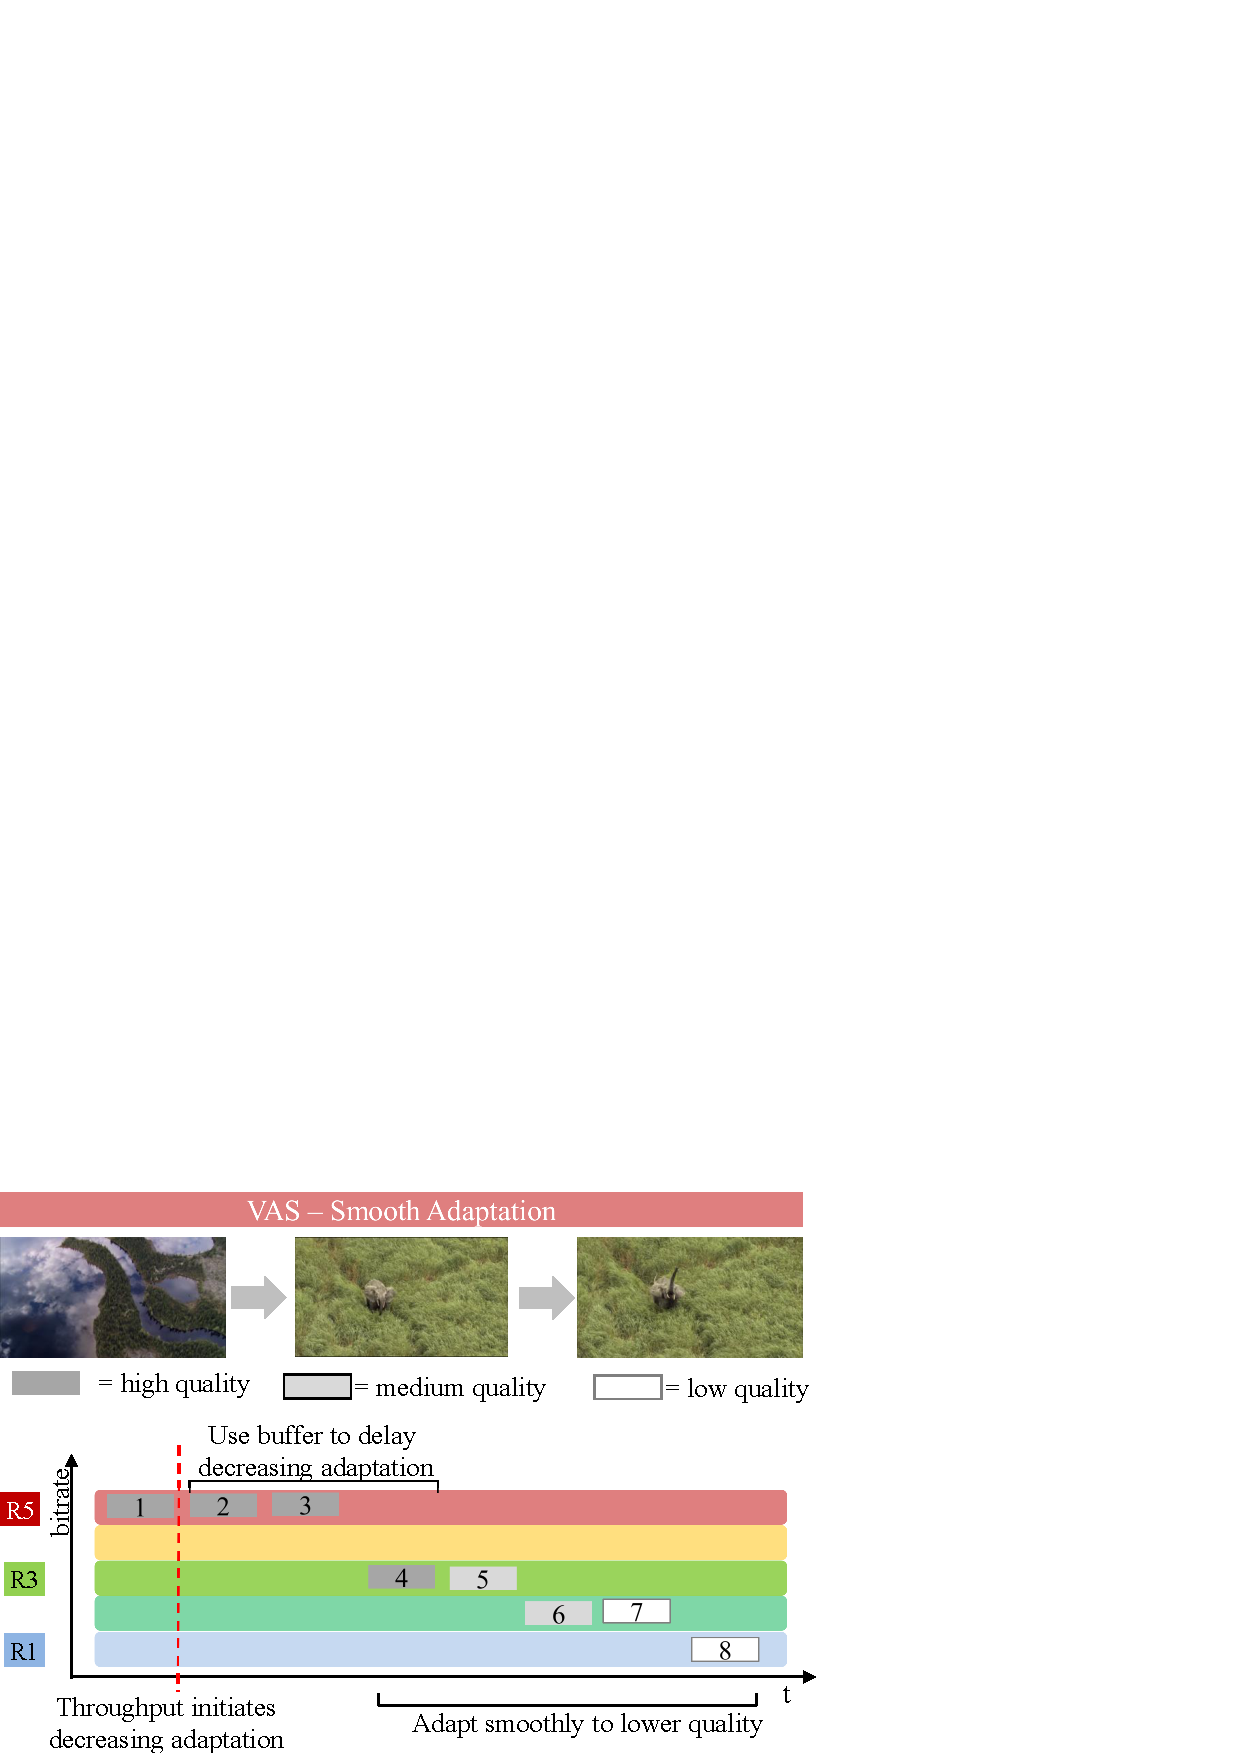
\includegraphics[width=\linewidth]{./gfx/700_VAS/smoothAdapt.pdf}
\caption{Example of using SQA as proposed by the \ac{VAS}.}
\label{fig:720_SmoothAdaptation}
\end{figure}
The core idea of the scheme is to \emph{slowly} adapt towards the target representation by integrating intermediate adaptations which are nearly unnoticeable.
\ac{VAS} relies on the findings of subjective studies of Moorthy et al., which offer thresholds on the perception of quality differences on mobile device displays~\cite{Moorthy2012}.
Also, the playback buffer is leveraged to delay adaptation as much as possible, to keep the streaming experience high without risking stalling effects.
The playback of video streaming at the highest quality representation has been shown to be beneficial~\cite{Hossfeld2014,Moorthy2012}.
It leverages both the available buffer and the current throughput to determine the point when the complete adaptation must be completed.
To reduce the risk of \ac{stalling}, the threshold $B_{c}$ is defined, which limits the amount of buffered data to be used for delaying the adaptation.

In a second step, an adaptation model is chosen by \ac{VAS}, which represents the perceived qualities between the current and target representations. 
All intermediate representations are skipped until the representation with the index $i$ is found which lies between the source representation $R_S$ and target representation $R_T$.
Thus, for an adaptation with quality decrease, the following condition must hold: $R_S > R_i > R_T$.

The representation $i$ is chosen so that the quality difference is nearly unnoticeable: $Q_{R_i} - Q_{R_S}  < Q_{ND}$, where $Q_{ND}$ is the \ac{MOS} value that defines a barrier when an adaptation between two representations is perceivable for the given content characteristics.
This step is repeated for as many intermediate adaptations as necessary. The generalized function can be represented $Q_{R_i} - Q_{R_{RLV}}  < Q_{ND}$, where $R_{RLV}$ represents the representation which was visited in the last planned adaptation.
The $Q_{ND}$ values for different combinations are backed by the dataset provided by Moorthy et al.~\cite{Moorthy2012}. 
In the experiments, $Q_{ND}$ usually ranges between 0.05 and 0.19.

Ideally, this approach results in a list of unnoticeable adaptations between a source representation and a target representation, called the adaptation plan $P_{S,T}$.
As those adaptations can be triggered by a decrease in network throughput, the danger of stalling is imminent if too many adaptations are conducted over a time period.
As stalling events usually severely degrade the perceived quality, it is the aim to avoid their occurrence during a streaming session~\cite{VanKester2011}.
A time constraint is defined based on the available buffer fill state ($FR_{B}$), the measured throughput ($TP_{t}$) and the bit rate of the current \ac{MPEG} \ac{DASH} representation ($BR_{R_i}$):
\begin{equation}
t_{P_{S,T}} = (FR_{B} - B_{c} * t_{B_{max}}) \times (1+\frac{TP_{t}}{BR_{R_i}}) \quad \mbox{in\quad [s]}
\end{equation}
Here, $B_{c}$ represents the fraction of the complete buffer length ($t_{B_{max}}$) that is preserved to ensure continuous playback.

For each adaptation at index $j$ in $P_{S,T}$ the time of the adaptation $t_j$ is determined by:
\begin{equation}
t_j = t + j * \frac{t_{P_{S,T}}}{N_{P_{S,T}}}
\end{equation}
$N_{P_{S,T}}$ is the number of necessary adaptations.

Adaptations are distinguished between those that aim at decrease the quality level and those that increase it.
The aforementioned approach is valid for decreasing adaptations.
Following the findings of Hossfeld et al. and Moorthy et al., \ac{VAS} aims to stay at high-quality representations as long as possible but also smoothly adapt to lower representations~\cite{Hossfeld2014,Moorthy2012}.
Furthermore, Lewcio et al. show that a quality-increasing adaptation improves the streaming experience~\cite{Lewcio2011}.
Thus, \ac{VAS} performs a direct jump from the source to the target representation for a quality-increasing adaptation.
%===========================================================================
\subsection{Integration into Existing Adaptation Schemes}
\label{sec:726_adaptation_strategies}
The concept of \ac{VAS} is to support existing adaptation schemes that solely consider the current network conditions or the playback buffer level, in adapting in a content- and quality-aware manner.
As mentioned, \ac{VAS} does not introduce a new throughput-related adaptation scheme, but it can be plugged into existing adaptation modules of \ac{MPEG} \ac{DASH} streaming clients (as depicted in Figure~\ref{fig:vasclientintegration}).

\begin{figure}
\centering
\includegraphics[width=0.98\linewidth]{gfx/700_VAS/VAS_CLIENT_INTEGRATION}
\caption{Integration of VAS adaptation schemes.}
\label{fig:vasclientintegration}
\end{figure} 
The decision of the adaptation scheme introduced by the \ac{MPEG} \ac{DASH} client is used as an upper bound for the \ac{VAS} decision, i.e., the maximum bit rate to be selected by the \ac{VAS} adaptation scheme.
The decision of which representation to choose is based on comparing throughput conditions of the network, the current playback buffer fill state, or a combination of both metrics.
As a result, one representation, and an optional timestamp when to switch, are the output of \ac{VAS} to the client. 

The client's \ac{VAS} component leverages information of the bit rate of the recommended adaptation and makes it an upper bound. 
The upper bound is known as $r_{t,max}$, where $r$ represents the representation index, $max$ depicts the highest representation index to be selected, and $t$ depicts the current timestamp.
The adaptation plan generated by \ac{VAS} does not include any representation with a higher bit rate; however, \ac{VAS} first applies the \ac{TQA} to select a representation with a lower bit rate which offers the desired quality level of the streaming session or an equal (or higher quality) than $r_{t,max}$.
As the quality may change over upcoming video shots, \ac{VAS} gives an adaptation plan to the adaptation execution component, which may consist of a list of representations to switch to and the adaptation timestamps.